\documentclass[12pt,a4paper]{article}

% Essential packages
\usepackage{graphicx}
\usepackage{setspace}
\usepackage[numbers,sort&compress]{natbib}
\usepackage[english]{babel}
\usepackage[utf8]{inputenc}
\usepackage{color}
\usepackage{hyperref}
\usepackage{amsmath,amssymb}
\usepackage{geometry}
\usepackage{longtable}
\usepackage{caption}
\usepackage{tikz}
\usepackage{adjustbox}
\usepackage{listings}
\usepackage{xcolor}
\usepackage{booktabs}
\usepackage{multirow}
\usepackage{float}
\usepackage{subcaption}
\usetikzlibrary{arrows.meta, positioning, shapes.geometric, calc, fit, backgrounds}

% Code listing configuration
\lstset{
    basicstyle=\ttfamily\small,
    breaklines=true,
    frame=single,
    backgroundcolor=\color{gray!10},
    keywordstyle=\color{blue},
    commentstyle=\color{green!50!black},
    stringstyle=\color{red!60!black},
    numbers=left,
    numberstyle=\tiny\color{gray},
    numbersep=5pt,
    showstringspaces=false,
    tabsize=2
}

\lstdefinelanguage{Python}{
    keywords={def, class, return, if, else, elif, for, while, with, as, import, from, async, await, try, except, finally, raise, True, False, None, and, or, not, in, is, lambda, yield},
    keywordstyle=\color{blue}\bfseries,
    ndkeywords={self, cls, BaseModel, Field, Literal, Optional, Union, list, dict, str, int, float, bool},
    ndkeywordstyle=\color{purple},
    sensitive=true,
    comment=[l]{\#},
    morestring=[b]",
    morestring=[b]',
}

% Margin settings
\geometry{
    a4paper,
    left=3cm,
    right=2.5cm,
    top=2.5cm,
    bottom=2.5cm
}

% Hyperref configuration
\hypersetup{
    colorlinks=true,
    linkcolor=blue,
    citecolor=blue,
    urlcolor=blue,
    pdftitle={Materials and Methods - Multi-Agent System for Fact-Checking},
    pdfauthor={Begoña Echavarren Sánchez}
}

% Spacing
\onehalfspacing

\begin{document}

\begin{titlepage}
    \begin{center}
    \vspace*{0.5cm}

    \includegraphics[width=0.6\textwidth]{../../assets/uoc_logo.png}

    \vspace{1.5cm}

    {\Huge \textbf{Materials, Methods and Results}}

    \vspace{2cm}

    {\LARGE \textbf{Multi-Agent System for Automated Fact-Checking of YouTube Videos}}

    \vspace{2.5cm}

    \textbf{\large Begoña Echavarren Sánchez}

    \vspace{0.5cm}

    \textit{Tutor: Josep-Anton Mir Tutusaus}

    \vspace{2cm}

    {\large Master's Degree in Data Science}

    {\large Universitat Oberta de Catalunya}

    \vspace{1cm}

    {\large PEC 3 - Implementation}

    \vspace{0.5cm}

    {\large December 2025}

    \end{center}
\end{titlepage}

\newpage
\pagenumbering{arabic}

\hypersetup{linkcolor=black}
\tableofcontents
\hypersetup{linkcolor=blue}

\newpage

%%%%%%%%%%%%%%%%%%%%%%%%%%%%%%%%%%%%%%%%%%%%%%%%%%%%%%%
% SECTION 1: MATERIALS AND METHODS
%%%%%%%%%%%%%%%%%%%%%%%%%%%%%%%%%%%%%%%%%%%%%%%%%%%%%%%
\section{Materials and Methods}

This section presents the comprehensive technical implementation of Factible, a multi-agent system for automated fact-checking of YouTube videos. The complete source code is publicly available at \url{https://github.com/begoechavarren/factible}. The system implements an end-to-end pipeline that processes video content through five specialized components, leveraging large language models (LLMs) for reasoning tasks while employing classical algorithms for deterministic operations. The implementation follows design-science principles \citep{hevner2004design, oates2006researching} and focuses on building practical artifacts that are iteratively evaluated and refined.

%-------------------------------------------------------
\subsection{System Architecture Overview}
%-------------------------------------------------------

\subsubsection{High-Level Architecture}

Factible implements an end-to-end automated fact-checking pipeline for YouTube videos using a multi-agent architecture. Recent research on LLM agents demonstrates that multi-agent collaboration can enhance factuality and reasoning by allowing specialized agents to coordinate on tasks \citep{wu2023autogen}. FactAgent further shows that decomposing fact-checking into dedicated agents for input ingestion, query generation, evidence retrieval, and verdict prediction yields higher accuracy and transparency \citep{zhang2025factagent}. The Factible architecture follows this line of work by processing video content through five specialized, modular components that operate sequentially with three levels of internal parallelization.

The system processes a YouTube video URL through five sequential stages, each with specialized responsibilities. The pipeline begins with transcript extraction, proceeds through claim and query generation, conducts online evidence retrieval, and culminates in structured verdict synthesis. This modular design enables independent optimization of each component while maintaining clear data contracts between stages.

The five stages are:

\begin{enumerate}
    \item \textbf{Transcriptor}: Extracts video transcripts via YouTube Transcript API, preserving timestamped segments for claim localization. The component includes automatic fallback to proxy service when rate-limited, ensuring robust transcript retrieval across different access conditions.

    \item \textbf{Claim Extractor} (LLM Agent): Employs thesis-first reasoning to infer the video's central argument before extracting factual and verifiable claims. Each claim receives an importance score based on its impact on the video's thesis. Post-processing uses fuzzy string matching to locate claims within the transcript for timestamp mapping.

    \item \textbf{Query Generator} (LLM Agent): Generates diverse search queries across four strategic types---direct, alternative, source-seeking, and contextual. Each query receives a priority score (1--5) based on evidence likelihood, enabling filtering of low-priority queries.

    \item \textbf{Online Search}: Executes a four-step evidence retrieval pipeline for each query: (i) Google Search via Serper API, (ii) website reliability assessment using Media Bias/Fact Check (MBFC) data combined with domain heuristics \citep{mbfc2024methodology}, (iii) content fetching via Selenium WebDriver with JavaScript rendering support, and (iv) LLM-based evidence extraction with stance classification (supports, refutes, mixed, unclear).

    \item \textbf{Output Generator} (LLM Agent): Synthesizes evidence into structured verdicts by building evidence bundles grouped by stance, generating natural language summaries with confidence levels, calculating algorithmic evidence quality scores, and mapping claims to video timestamps for interactive navigation.
\end{enumerate}

Figure \ref{fig:pipeline-architecture} illustrates the complete pipeline architecture with data flow and parallelization points across all five stages.

\begin{figure}[H]
\centering
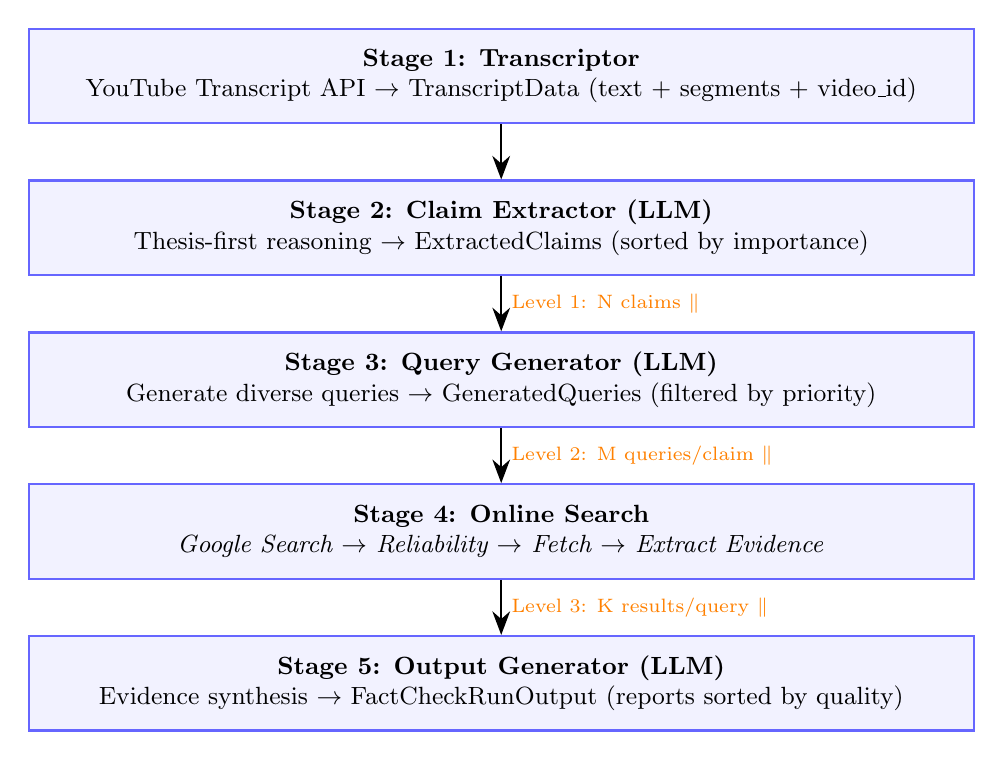
\begin{tikzpicture}[
    node distance=0.7cm,
    box/.style={rectangle, draw=blue!60, fill=blue!5, thick, minimum width=12cm, minimum height=1.2cm, align=center, font=\small},
    arrow/.style={-{Stealth[length=3mm]}, thick},
    parallel/.style={draw=orange!70, dashed, thick}
]

% Stage 1
\node[box] (s1) {
    \textbf{Stage 1: Transcriptor}\\
    YouTube Transcript API $\rightarrow$ TranscriptData (text + segments + video\_id)
};

% Stage 2
\node[box, below=of s1] (s2) {
    \textbf{Stage 2: Claim Extractor (LLM)}\\
    Thesis-first reasoning $\rightarrow$ ExtractedClaims (sorted by importance)
};

% Stage 3
\node[box, below=of s2] (s3) {
    \textbf{Stage 3: Query Generator (LLM)}\\
    Generate diverse queries $\rightarrow$ GeneratedQueries (filtered by priority)
};

% Stage 4
\node[box, below=of s3] (s4) {
    \textbf{Stage 4: Online Search}\\
    \textit{Google Search $\rightarrow$ Reliability $\rightarrow$ Fetch $\rightarrow$ Extract Evidence}
};

% Stage 5
\node[box, below=of s4] (s5) {
    \textbf{Stage 5: Output Generator (LLM)}\\
    Evidence synthesis $\rightarrow$ FactCheckRunOutput (reports sorted by quality)
};

% Arrows
\draw[arrow] (s1) -- (s2);
\draw[arrow] (s2) -- node[right, font=\scriptsize, orange] {Level 1: N claims $\parallel$} (s3);
\draw[arrow] (s3) -- node[right, font=\scriptsize, orange] {Level 2: M queries/claim $\parallel$} (s4);
\draw[arrow] (s4) -- node[right, font=\scriptsize, orange] {Level 3: K results/query $\parallel$} (s5);

\end{tikzpicture}
\caption{High-level pipeline architecture showing the five main stages and three parallelization levels. Parallelization occurs at claims (Level 1), queries per claim (Level 2), and search results per query (Level 3). Verdict generation happens within Level 1 after each claim's evidence is collected.}
\label{fig:pipeline-architecture}
\end{figure}

\subsubsection{Design Principles}

The system adheres to several key design principles derived from software engineering best practices and GenAI application development \citep{hevner2004design}:

\begin{enumerate}
    \item \textbf{Modularity}: Each component is isolated with well-defined inputs and outputs using Pydantic schemas, enabling independent optimization, testing, and replacement.

    \item \textbf{Structured Outputs}: All LLM interactions use Pydantic AI with typed output schemas, ensuring type safety, automatic validation, and consistent data structures across the pipeline.

    \item \textbf{Transparency}: The full evidence chain is preserved and exposed to users---sources, reliability ratings, stances, and reasoning are all traceable from final verdict back to original source.

    \item \textbf{Progressive Enhancement}: The pipeline operates with graceful degradation (e.g., fallback to snippet if scraping fails, fallback to proxy if rate-limited) rather than failing entirely.

    \item \textbf{Cost-Conscious Design}: Configurable limits (\texttt{max\_claims}, \texttt{max\_queries}, \texttt{max\_results}) prevent runaway API costs and controled latency during development and production.

    \item \textbf{Reproducibility}: Deterministic LLM outputs (\texttt{temperature=0.0}), structured YAML configurations, and comprehensive experiment tracking enable reproducible research.

    \item \textbf{Separation of Concerns}: Classical algorithms handle tasks like reliability scoring, deduplication, and quality calculation, reserving LLM calls for tasks requiring reasoning and language understanding.
\end{enumerate}

\subsubsection{Component Isolation Pattern}

Each component follows a consistent structure that promotes modularity and maintainability. This standardized organization enables independent testing of each component in isolation, swapping LLM models for experimentation, automated metrics collection via decorators, and clear interface contracts through Pydantic schemas. The separation of concerns facilitates parallel development and reduces coupling between pipeline stages.

%-------------------------------------------------------
\subsection{Technology Stack}
%-------------------------------------------------------

\subsubsection{Core Technologies}

Table \ref{tab:tech-stack} presents the core technologies employed in the implementation.

\begin{table}[H]
\centering
\caption{Core technology stack}
\label{tab:tech-stack}
\begin{tabular}{llll}
\toprule
\textbf{Category} & \textbf{Technology} & \textbf{Version} & \textbf{Purpose} \\
\midrule
Language & Python & 3.12 & Core implementation with type hints \\
LLM Framework & Pydantic AI & $\geq$1.0.0 & Agent orchestration, structured outputs \\
Data Validation & Pydantic & $\geq$2.0.0 & Schema definitions, runtime validation \\
Web Framework & FastAPI & $\geq$0.115.0 & REST API with SSE streaming \\
HTTP Server & Uvicorn & $\geq$0.32.0 & High-performance ASGI server \\
Async HTTP & httpx & $\geq$0.28.1 & Async HTTP client \\
Web Scraping & Selenium & $\geq$4.15.2 & JavaScript-rendered content extraction \\
YouTube & youtube-transcript-api & $\geq$1.2.2 & Transcript extraction \\
Domain Info & python-whois & $\geq$0.8.0 & Domain age lookup \\
CLI & Typer & $\geq$0.15.0 & Experiment runner CLI \\
Analysis & pandas, matplotlib & - & Data analysis and visualization \\
\bottomrule
\end{tabular}
\end{table}

\subsubsection{Large Language Models}

The system supports multiple LLM providers to enable comparison of cost-quality trade-offs. Table \ref{tab:llm-models} shows the available models and their configurations.

\begin{table}[H]
\centering
\caption{LLM providers and pricing}
\label{tab:llm-models}
\begin{tabular}{lllll}
\toprule
\textbf{Provider} & \textbf{Model} & \textbf{Context} & \textbf{Pricing (per 1M tokens)} & \textbf{Use Case} \\
\midrule
OpenAI & gpt-4o-mini & 128K & \$0.15 / \$0.60 & Default \\
OpenAI & gpt-4o & 128K & \$5.00 / \$15.00 & High-quality \\
OpenAI & gpt-4-turbo & 128K & \$10.00 / \$30.00 & Premium \\
Ollama & qwen3:8b & 40K & Free (local) & Budget/offline \\
Ollama & qwen3:4b & 256K & Free (local) & Budget/offline \\
\bottomrule
\end{tabular}
\end{table}

Large language models such as GPT-4 offer multimodal capabilities and demonstrate human-level performance across diverse benchmarks \citep{openai2024gpt4}. Despite these advances, models still suffer from hallucinations and are constrained by limited context windows, underscoring the need for careful configuration and reliability safeguards \citep{openai2024gpt4}. The model management layer therefore makes it straightforward to switch providers, tune limits, and keep outputs deterministic through shared configuration.

The same layer also exposes a zero-cost, offline alternative through Ollama with three Qwen 3 variants (qwen3:8b, qwen3:4b, qwen3:1.7b). Switching between OpenAI and local providers requires only a configuration change, enabling experiments that balance latency, quality, and hardware constraints. GPT-4o-mini remains the default selection for this thesis because cloud inference provides lower latency than consumer hardware while maintaining strong reasoning quality.

\subsubsection{External Services}

The system integrates with external services for search and transcript extraction:

\begin{itemize}
    \item \textbf{Serper API}: Google Search wrapper providing organic search results with approximately 2,500 queries per month on the free tier.
    \item \textbf{YouTube oEmbed API}: Video metadata retrieval without authentication.
    \item \textbf{Webshare Proxy}: Rate limit bypass for transcript extraction with configurable proxy locations.
\end{itemize}

%-------------------------------------------------------
\subsection{Pipeline Components}
%-------------------------------------------------------

\subsubsection{Transcriptor}

The Transcriptor component extracts YouTube video transcripts with precise timestamp information for later claim-to-video mapping.

\paragraph{Implementation Details}

The transcriptor uses the \texttt{youtube-transcript-api} library to fetch available transcripts, with preference for English. When rate-limited by YouTube, it automatically falls back to a proxy service (Webshare). Key features include:

\begin{itemize}
    \item \textbf{Timestamped Segments}: Each segment preserves \texttt{start} time and \texttt{duration} in seconds.
    \item \textbf{Character Position Mapping}: Enables mapping claim text positions back to video timestamps.
    \item \textbf{Title Fetching}: Uses YouTube oEmbed API to retrieve video title for context.
    \item \textbf{Proxy Fallback}: Automatic retry through Webshare proxy when rate-limited.
\end{itemize}

\paragraph{Output and Timestamp Mapping}

Each run returns the video identifier, the full transcript text, and a list of timestamped segments containing text, start time, and duration. A lightweight mapping pass scans the segments sequentially while maintaining a cumulative character counter so that claim positions can be translated into timestamps. This enables the interface to jump straight to the moment where a claim appeared without duplicating transcript parsing logic elsewhere.

%---

\subsubsection{Claim Extractor}

The Claim Extractor identifies factual, verifiable claims from video transcripts using LLM-based extraction with thesis-relative importance ranking. This approach builds on prior work in automated claim detection: supervised models trained on annotated political debates have been used to detect check-worthy claims \citep{hassan2015claimbuster}, and end-to-end systems like ClaimBuster monitor public discourse and prioritize factual statements for manual fact-checking \citep{li2017claimbuster}. These systems show that focusing on salient, verifiable claims improves the efficiency of fact-checking pipelines.

\paragraph{LLM Configuration}

The claim extractor uses deterministic settings for reproducibility: temperature set to 0.0 to ensure consistent outputs across multiple runs, max tokens limited to 1,200 to control response length and latency, and automatic retry logic (3 attempts) to handle transient LLM failures gracefully.

\paragraph{Prompt Engineering Strategy: Thesis-First Approach}

The claim extractor employs a novel \textit{thesis-first approach} with multi-step reasoning designed to prioritize claims most critical to the video's central argument:

\textbf{Step 1: Thesis Inference} --- Before listing claims, the LLM infers the video's central thesis in no more than 25 words (e.g., ``Climate change alarmism is driven more by politics and media than by settled science'').

\textbf{Step 2: Importance Ranking with Thesis Impact Test} --- Claims are scored based on their impact on the video's thesis using the question: ``If this claim were proven false, would the thesis collapse or materially weaken?'' Table \ref{tab:importance-scoring} presents the scoring guidelines.

\begin{table}[H]
\centering
\caption{Claim importance scoring guidelines}
\label{tab:importance-scoring}
\small
\begin{tabular}{p{2.5cm}p{5.5cm}p{5cm}}
\toprule
\textbf{Score Range} & \textbf{Description} & \textbf{Examples} \\
\midrule
0.85--1.0 & Prescriptive/causal claims undermining thesis & Policy proposals, causal mechanisms \\
0.60--0.80 & Quantitative/historical evidence tied to thesis & Statistics, dates, expert citations \\
0.30--0.55 & Context/supporting background & Definitions, general facts \\
0.0--0.25 & Peripheral/anecdotal details & Personal stories, credentials \\
\bottomrule
\end{tabular}
\end{table}

\textbf{Step 3: Relevance Guardrails} --- Pure credential facts are capped at 0.30 unless the thesis questions expertise; statements not affecting the thesis are capped at 0.25; pure opinions are excluded; and paraphrases and duplicate numbers are removed.

\paragraph{Prompt Engineering Techniques}

The system employs several established prompting techniques across its components:

\begin{itemize}
    \item \textbf{Role/system prompting}: Each component receives a focused system prompt that spells out its role, constraints, and expected outputs for consistent behavior.
    \item \textbf{Structured outputs}: Responses are constrained to typed schemas so downstream stages always receive validated fields.
    \item \textbf{Chain-of-thought reasoning}: The thesis-first steps require the model to state the thesis and then rate claims against it, which improves prioritization.
    \item \textbf{Dynamic instruction injection}: Runtime parameters such as \texttt{max\_claims} are inserted directly into prompts so component behavior adapts without duplicating templates.
    \item \textbf{Deterministic generation}: Temperature stays at 0.0 across the pipeline for reproducible, debuggable outputs.
    \item \textbf{Zero-shot prompting}: Components receive task instructions without example I/O pairs, minimizing prompt length and avoiding format bias.
\end{itemize}

\paragraph{Post-Processing: Fuzzy Claim Localization}

After LLM extraction, each claim is located in the original transcript using fuzzy string matching. The algorithm normalizes both the claim text and transcript, then applies a sliding window approach (with $\pm 2$ words tolerance around the expected claim length) to find the best matching region. Similarity is computed using Python's sequence matching algorithm, which calculates the ratio of matching characters between two strings. A minimum similarity score of 0.5 is required for a valid match. This process yields the character-level start and end positions within the transcript, along with the match confidence score, enabling precise timestamp mapping from transcript positions back to video timestamps.

\paragraph{Output Schema}

Extracted claims are represented as structured objects with validated fields: claim text (recommended maximum 40 words), confidence score (0.0--1.0), category (historical, scientific, statistical), importance score (0.0--1.0), and optional context. Post-processing adds transcript location metadata including character positions and fuzzy match scores. The collection of claims is sorted by importance in descending order.

%---

\subsubsection{Query Generator}

The Query Generator produces diverse, prioritized search queries tailored to each claim. A single LLM call emits direct restatements, synonym-heavy variations, source-focused prompts, and broader context queries together with priority tags so downstream steps can respect latency budgets. Guardrails ensure the suggestions include relevant entities, time periods, and qualifiers while capping each claim at a manageable number of high-yield searches.

\paragraph{Query Type Taxonomy}

The system generates four types of queries with different search strategies, as shown in Table \ref{tab:query-types}.

\begin{table}[H]
\centering
\caption{Query type taxonomy}
\label{tab:query-types}
\small
\begin{tabular}{p{2.3cm}p{4cm}p{3cm}p{4cm}}
\toprule
\textbf{Type} & \textbf{Description} & \textbf{Strategy} & \textbf{Example} \\
\midrule
DIRECT & Exact claim phrasing & Verbatim search & ``unemployment rose 15\% Q3 2024'' \\
ALTERNATIVE & Rephrased with synonyms & Semantic variation & ``jobless rate increase third quarter'' \\
SOURCE & Target authoritative sources & Source-seeking & ``BLS unemployment statistics Q3'' \\
CONTEXT & Broader context & Background search & ``economic indicators fall 2024'' \\
\bottomrule
\end{tabular}
\end{table}

\paragraph{Priority System}

Queries are prioritized 1--5 based on likelihood of finding reliable, definitive information: priority 1 queries are always included, priority 2 by default, priority 3 if budget allows, and priorities 4--5 rarely or only for completeness.

\paragraph{Context-Aware Query Generation}

Beyond factual accuracy, the query generator is designed to detect misleadingly framed claims---statements that may be technically accurate but presented without essential context. The system prompt instructs the LLM to respect temporal context when choosing keywords (e.g., including relevant years or qualifiers to avoid mixing eras), and to explicitly generate queries seeking counter-arguments or opposing views. This approach helps surface evidence that may qualify, limit, or contextualize the original claim, enabling more nuanced verdict generation. For example, a claim stating ``unemployment dropped 20\%'' might be technically accurate for a specific quarter but misleading without the broader trend; context-aware queries would seek both confirming statistics and broader economic context.

\paragraph{Output Schema}

Generated queries are structured objects containing the query text, query type (direct, alternative, source, or context), and priority (1--5, with 1 being highest). The complete output includes the original claim reference, a filtered and sorted list of queries, and a count of total queries generated before filtering.

%---

\subsubsection{Online Search}

The Online Search component implements a multi-step pipeline to retrieve, assess, and extract evidence from web sources with adaptive quality filtering. Unlike the other LLM-based components, Online Search orchestrates multiple classical algorithms alongside a single LLM call for evidence extraction. This hybrid approach balances speed, reliability, and reasoning capabilities.

The reliability assessment combines domain-level heuristics with the Media Bias/Fact Check (MBFC) methodology, which employs a comprehensive weighted scoring system to evaluate media outlets' ideological bias and factual reliability \citep{mbfc2024methodology}. These scores, combined with stance-aware evidence extraction instructions, keep unreliable or speculative passages from flowing downstream.

Figure \ref{fig:online-search-pipeline} illustrates the four-step Online Search pipeline executed for each query.

\begin{figure}[H]
\centering
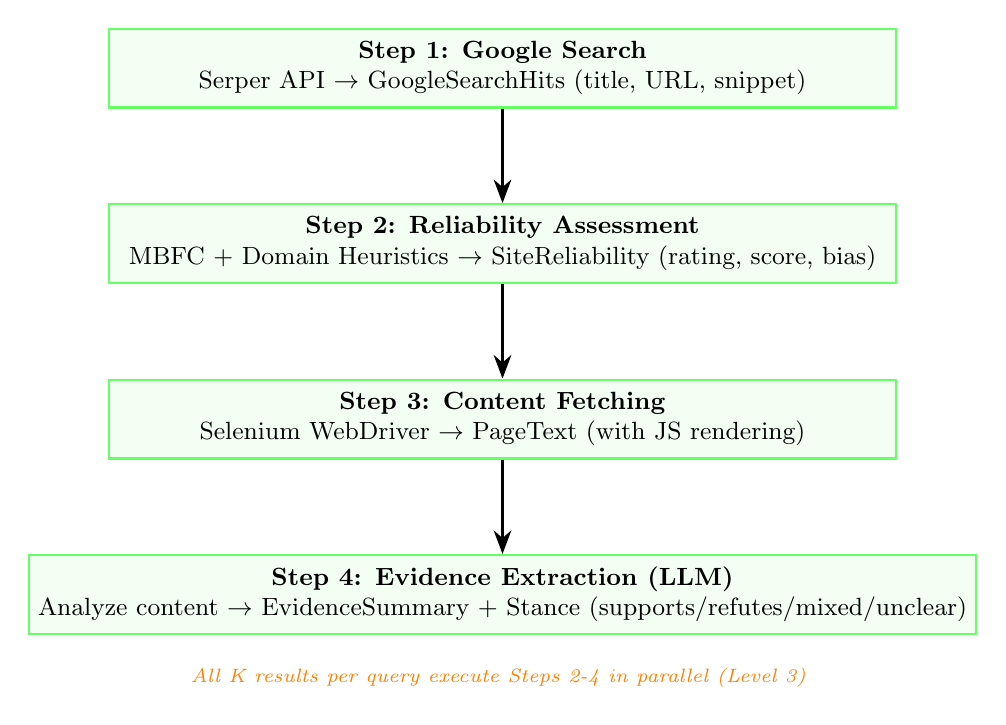
\begin{tikzpicture}[
    node distance=1.2cm,
    box/.style={rectangle, draw=green!60, fill=green!5, thick, minimum width=10cm, minimum height=1cm, align=center, font=\small},
    arrow/.style={-{Stealth[length=3mm]}, thick},
]

% Step 1
\node[box] (step1) {
    \textbf{Step 1: Google Search}\\
    Serper API $\rightarrow$ GoogleSearchHits (title, URL, snippet)
};

% Step 2
\node[box, below=of step1] (step2) {
    \textbf{Step 2: Reliability Assessment}\\
    MBFC + Domain Heuristics $\rightarrow$ SiteReliability (rating, score, bias)
};

% Step 3
\node[box, below=of step2] (step3) {
    \textbf{Step 3: Content Fetching}\\
    Selenium WebDriver $\rightarrow$ PageText (with JS rendering)
};

% Step 4
\node[box, below=of step3] (step4) {
    \textbf{Step 4: Evidence Extraction (LLM)}\\
    Analyze content $\rightarrow$ EvidenceSummary + Stance (supports/refutes/mixed/unclear)
};

% Arrows
\draw[arrow] (step1) -- (step2);
\draw[arrow] (step2) -- (step3);
\draw[arrow] (step3) -- (step4);

% Parallelization note
\node[below=0.3cm of step4, font=\scriptsize, orange, align=center] {
    \textit{All K results per query execute Steps 2-4 in parallel (Level 3)}
};

\end{tikzpicture}
\caption{Online Search pipeline showing the four sequential steps executed for each search result. Steps 2--4 run in parallel across all K results per query (Level 3 parallelization).}
\label{fig:online-search-pipeline}
\end{figure}

\paragraph{Step 1: Google Search (Serper API)}

The Google search client wraps the Serper API for asynchronous search execution. The implementation uses persistent HTTP connections for performance and returns structured search hits containing title, URL, and snippet fields. Each query can retrieve up to 10 results, with the limit parameter controlling the exact number returned. The async design enables parallel query execution across multiple claims simultaneously.

\paragraph{Step 2: Website Reliability Assessment}

The reliability checker uses a multi-factor scoring system with first-match priority, combining external datasets with algorithmic heuristics:

\begin{itemize}
    \item \textbf{Media Bias/Fact Check (MBFC) Dataset}: The system loads timestamped JSON snapshots containing nearly 10,000 news sources with credibility ratings (dataset extracted December 2025). Credibility mappings are: high $\rightarrow$ 0.85, medium $\rightarrow$ 0.60, low $\rightarrow$ 0.30, very low $\rightarrow$ 0.15.

    \item \textbf{TLD Reputation}: High-trust top-level domains (\texttt{.gov}, \texttt{.edu}, \texttt{.int}) receive a base score of 0.90, reflecting their institutional authority.

    \item \textbf{Domain Age via WHOIS}: Domains $\geq$10 years old receive a +0.10 bonus (established presence), while domains $<$1 year old receive a --0.15 penalty (recent creation may indicate lower trust).
\end{itemize}

The output includes a categorical rating (high, medium, low, unknown), numerical score (0.0--1.0), reasoning for the assessment, and political bias classification when available from MBFC data.

\paragraph{Step 3: Content Fetching (Selenium)}

Content fetching uses headless Chrome with smart waits: the scraper first grabs paragraph elements immediately, then allows extra rendering time only when less than 100 characters were captured. Images are disabled, page-load and wait timeouts cap the work (20 seconds and 12 seconds, respectively), and the cleaned text is trimmed to 8,000 characters before being passed to the LLM. Blocking Selenium calls are delegated to background threads so multiple results can be processed in parallel without freezing the async loop.

\paragraph{Step 4: Evidence Extraction (LLM)}

The evidence extractor analyzes retrieved content against claims using structured stance definitions:

\begin{itemize}
    \item \textbf{SUPPORTS}: Evidence confirms or validates the claim through direct statements, semantic equivalents, or mechanism descriptions.
    \item \textbf{REFUTES}: Evidence contradicts or disproves the claim through counter-evidence or statements that evidence is unproven/disproven.
    \item \textbf{MIXED}: Both supporting and refuting elements present.
    \item \textbf{UNCLEAR}: Genuinely ambiguous content that discusses related topics without addressing the specific claim.
\end{itemize}

Critical prompt instructions ensure that mere discussion equals UNCLEAR, that mechanisms are recognized even without exact terminology, and that both Google snippets and page content are considered with better evidence prioritized. Importantly, the evidence extractor pays special attention to qualifiers such as ``only'', ``never'', ``always'', and temporal scope limitations (e.g., ``since X date'')---this enables detection of claims that may be technically accurate but misleadingly framed due to omitted context or overgeneralization.

\paragraph{Adaptive Credibility Filtering}

The search orchestrator implements adaptive credibility filtering as a key innovation for ensuring evidence quality. The algorithm operates in three phases:

\begin{enumerate}
    \item \textbf{Initial Batch}: Fetch 2× the desired limit to provide filtering margin
    \item \textbf{Quality Check}: If $>$50\% of results are unreliable, fetch an additional batch to increase the pool of high-quality sources
    \item \textbf{Intelligent Filtering}: Sort all results by reliability score and select the top reliable sources, with a minimum guarantee ensuring at least some results are returned even if reliability is universally low
\end{enumerate}

Additional filtering mechanisms include stance filtering (removing unclear results if $>$50\% have definitive stances) and URL deduplication using sets to prevent duplicate sources across different queries for the same claim.

%---

\subsubsection{Output Generator}

The Output Generator synthesizes evidence into coherent verdicts with confidence levels, quality scoring, and timestamp mapping.

\paragraph{Two-Step Process}

The Output Generator employs a hybrid approach combining algorithmic evidence organization with LLM-based synthesis:

\textbf{Step 1: Build Evidence Bundle (Algorithmic)} --- The system groups evidence by stance (supports, refutes, mixed, unclear), deduplicates sources by URL, and sorts within each group by reliability rating (high first), then numerical score, with alphabetic tie-breaking for consistency.

\textbf{Step 2: Generate Verdict (LLM)} --- Organized evidence is formatted into a structured prompt containing stance labels, source counts, reliability ratings, and evidence summaries. The system prompt instructs the LLM to synthesize concise verdicts, naming sources explicitly only when clarifying contrasting perspectives or when evidence directly conflicts. This reduces verbosity while maintaining attribution transparency.

\paragraph{Evidence Quality Score (Algorithmic)}

The quality score is calculated algorithmically without LLM involvement for consistency and speed. The scoring formula combines three components with different weights: a base score of 0.3 for having any evidence, an actionable stance bonus of up to 0.3 (scaled by the number of supports/refutes/mixed sources, saturating at 3 sources), and a reliability bonus of up to 0.4 (scaled by the number of high/medium reliability sources, saturating at 3 sources). This design prioritizes both actionable stances and source reliability, with the maximum achievable score of 1.0 indicating high-quality, decisive evidence from multiple reliable sources.

Table \ref{tab:quality-score} summarizes the quality score components.

\begin{table}[H]
\centering
\caption{Evidence quality score breakdown}
\label{tab:quality-score}
\begin{tabular}{lll}
\toprule
\textbf{Component} & \textbf{Weight} & \textbf{Criteria} \\
\midrule
Base & 0.3 & Having any evidence \\
Actionable & 0.3 & Up to 3 supports/refutes/mixed sources \\
Reliability & 0.4 & Up to 3 high/medium reliability sources \\
\textbf{Maximum} & \textbf{1.0} & \\
\bottomrule
\end{tabular}
\end{table}

\paragraph{Integrated Verdict Generation (within Level 1)}

Verdicts are generated immediately after each claim's evidence collection completes, within the same parallel execution context as the claim processing. This design choice eliminates the latency overhead of waiting for all claims to finish evidence collection before beginning verdict synthesis. Each claim's verdict generation executes as soon as its evidence is ready, allowing early-finishing claims to produce results while slower claims continue processing. After all parallel claim tasks complete, the reports are sorted by evidence quality score (descending) to prioritize high-confidence verdicts in the user interface.

\paragraph{Output Schema}

The fact-check report is a structured object containing all information for user presentation: claim metadata (text, confidence, category), verdict assessment (overall stance, confidence level, summary), evidence organization (grouped by stance with source summaries), quality metrics (total source count, evidence quality score), and optional timestamp references for video navigation. Verdict confidence is constrained to low, medium, or high levels.

%-------------------------------------------------------
\subsection{LLM Configuration and Model Management}
%-------------------------------------------------------

\subsubsection{Model Abstraction Layer}

All LLM settings live in a single configuration document that lists each provider, the model identifier, pricing information, and context window. Component modules refer only to that catalog, so swapping a model or updating prices requires editing one place rather than chasing hard-coded strings. The abstraction is deliberately simple—just structured data that the pipeline reads on startup—yet it keeps experiments reproducible because every run records the same model metadata.

\subsubsection{Per-Component Model Configuration}

Each pipeline stage points to a default cloud model for consistency, but any component can be redirected to a different provider through configuration alone. This granular setup enables per-component tests without touching code.

\subsubsection{Common Model Settings}

All components use \texttt{temperature=0.0} for deterministic outputs, enabling reproducibility, consistency in structured outputs, and meaningful comparisons. Table \ref{tab:model-settings} shows the token limits per component.

\begin{table}[H]
\centering
\caption{Component model settings}
\label{tab:model-settings}
\begin{tabular}{llll}
\toprule
\textbf{Component} & \textbf{Temperature} & \textbf{Max Tokens} & \textbf{Rationale} \\
\midrule
Claim Extractor & 0.0 & 1,200 & Deterministic, structured claims \\
Query Generator & 0.0 & 600 & Concise queries, no explanations \\
Evidence Extractor & 0.0 & 1,100 & Summary + key quote \\
Output Generator & 0.0 & 900 & Concise verdict synthesis \\
\bottomrule
\end{tabular}
\end{table}
%-------------------------------------------------------
\subsection{Latency Optimization Strategies}
%-------------------------------------------------------

The pipeline ships with a concrete set of latency optimizations inspired by LLM engineering guidelines but implemented specifically for Factible. The following subsections describe what was actually built: tuned model choices, strict token budgets, trimmed inputs, single-call components, parallel execution, real-time streaming updates, and classical fallbacks for non-reasoning tasks. Together these measures reduced mean end-to-end latency to 129.6 seconds for the current evaluation set.

\subsubsection{Process Tokens Faster: Model Selection}

The default model (gpt-4o-mini) is selected for its balanced performance across speed, cost-effectiveness, and large context window (128K tokens). This model provides sufficient reasoning capabilities for fact-checking tasks while maintaining low latency and competitive pricing (\$0.15 per million input tokens, \$0.60 per million output tokens). For budget-conscious deployments or offline operation, local Ollama models (qwen3:8b, qwen3:4b) offer zero-cost inference at the expense of potential quality degradation. The modular model abstraction layer enables easy comparison of these trade-offs through experiment configuration.

\subsubsection{Generate Fewer Tokens: Output Constraints}

Each component has carefully tuned \texttt{max\_tokens} limits to minimize generation latency and API costs without sacrificing information quality. Claims are limited to approximately 40 words (sufficient for most factual assertions), context descriptions to 20 words (brief background), and evidence summaries to 1--2 sentences (key findings only). These constraints are enforced through explicit prompt instructions and validated against output token limits. By preventing verbose outputs, the system reduces both generation time and downstream processing costs for subsequent pipeline stages.

\subsubsection{Use Fewer Input Tokens: Content Trimming}

Input token counts are minimized through aggressive content trimming strategies. Web content is trimmed to 6,000--8,000 characters before being passed to the Evidence Extractor, removing excessive context while retaining the most relevant portions (typically the first several paragraphs of an article). Evidence prompts include only Google snippets and extracted page text, explicitly excluding raw HTML, JavaScript, CSS, and other non-content elements that would inflate token counts without improving extraction quality. This targeted trimming reduces LLM input costs by an order of magnitude compared to naive full-page submission.

\subsubsection{Make Fewer Requests: Combined Operations}

The pipeline minimizes LLM API calls by combining operations into single requests wherever possible. Each component makes exactly one LLM call per input unit (one call for claim extraction, one per claim for query generation, one per search result for evidence extraction, and one per claim for verdict synthesis), with no multi-turn conversations that would multiply request counts. The Query Generator produces all queries for a claim in a single batch call rather than generating queries iteratively. Similarly, the Output Generator synthesizes verdicts with all available evidence in a single call. This design reduces API overhead, improves latency, and simplifies cost tracking.

\subsubsection{Parallelize: 3-Level Async Architecture}

The system implements three levels of nested parallelization to maximize throughput while maintaining dependency ordering. This architecture enables the pipeline to process multiple claims, queries, and search results simultaneously, dramatically reducing total execution time compared to sequential processing.

The parallelization hierarchy operates as follows:

\begin{itemize}
    \item \textbf{Level 1 (Claims)}: After extracting N claims from the transcript, all claims are processed in parallel. Each claim independently proceeds through query generation, evidence search, and verdict generation. Critically, each claim's verdict is generated immediately after its evidence collection completes, rather than waiting for all claims to finish---this optimization reduces perceived latency by producing results progressively.

    \item \textbf{Level 2 (Queries per Claim)}: Within each claim's processing, the Query Generator produces M queries. These queries are executed in parallel, enabling simultaneous search across different query formulations (direct, alternative, source-seeking, contextual).

    \item \textbf{Level 3 (Search Results per Query)}: Within each query's execution, the Online Search component retrieves K results from Google. The four-step pipeline (reliability assessment, content fetching, and evidence extraction) runs in parallel for all K results, with each result processed independently.
\end{itemize}

This design achieves maximum theoretical parallelization of $N \times M \times K$ operations during the search phase, bounded only by system resources and API rate limits. The nesting structure means that at peak execution, the system may be processing dozens of parallel operations across all three levels simultaneously. Blocking I/O operations (Selenium WebDriver for content fetching, WHOIS for domain age lookup) are delegated to worker threads to keep the async event loop responsive, ensuring that CPU-bound and I/O-bound operations can execute concurrently.

\subsubsection{Real-Time Streaming}

Server-Sent Events (SSE) provide progressive updates as the pipeline executes, improving perceived responsiveness for users. Each update labels the active stage (e.g., ``claim extraction'', ``processing\_claim\_2'', ``generating\_report'') alongside a percentage so the UI can display the exact component currently running. Extracted claims are streamed immediately after the Claim Extractor finishes, enabling preview and early user feedback while later stages gather evidence. This progressive disclosure pattern reduces perceived latency and gives users clear visibility into pipeline progress.

\subsubsection{Classical Methods for Non-Reasoning Tasks}

Table \ref{tab:classical-methods} shows operations handled by classical algorithms rather than LLMs.

\begin{table}[H]
\centering
\caption{Operations using classical methods}
\label{tab:classical-methods}
\begin{tabular}{lll}
\toprule
\textbf{Operation} & \textbf{Method} & \textbf{Rationale} \\
\midrule
Reliability scoring & Rule-based + MBFC lookup & Faster, deterministic, no API cost \\
Claim localization & Fuzzy string matching & No LLM needed for text search \\
Evidence quality score & Algorithmic calculation & Consistent, fast, reproducible \\
URL deduplication & Hash set & O(1) lookup \\
Stance filtering & Threshold-based & Simple percentage check \\
\bottomrule
\end{tabular}
\end{table}

%-------------------------------------------------------
\subsection{Structured Outputs with Pydantic}
%-------------------------------------------------------

All LLM agents use Pydantic models to constrain their outputs, providing comprehensive type safety throughout the pipeline. This approach offers several benefits for LLM-based systems:

\begin{itemize}
    \item \textbf{Reliable parsing}: LLM outputs are automatically parsed and validated against the schema, eliminating manual JSON handling and catching malformed responses immediately.
    \item \textbf{Automatic retries}: When the LLM produces invalid output (e.g., missing required fields, out-of-range values), Pydantic AI automatically retries with feedback about the validation error.
    \item \textbf{Clear contracts}: Schemas define explicit interfaces between pipeline stages, enabling independent development and testing of each component.
    \item \textbf{Reduced hallucination}: Constraining outputs to predefined structures (e.g., stance must be one of four values) prevents the LLM from inventing invalid categories or formats.
\end{itemize}

This declarative configuration style reduces boilerplate while maintaining explicit control over agent behavior, and ensures robust data flow across the entire pipeline.

%-------------------------------------------------------
\subsection{Experimentation and Evaluation Framework}
%-------------------------------------------------------

Evaluating LLM-based fact-checking systems presents unique challenges: outputs are non-deterministic, external dependencies (web search) introduce variability, and traditional benchmarks risk overfitting \citep{ruder2025evolving}. To address these challenges, a three-component experimentation framework was developed to capture complete execution traces, support batch experimentation, and compute performance metrics.

\subsubsection{Framework Architecture}

The framework follows a linear data flow through three stages:

\begin{enumerate}
    \item \textbf{Experiment Runner}: Executes the fact-checking pipeline on configured videos, invoking the tracking module for each run.
    \item \textbf{Tracking Module}: Captures all execution data---inputs, outputs, LLM calls, timing, and costs---saving structured artifacts for later analysis.
    \item \textbf{Evaluator}: Computes performance metrics including comparisons against ground truth annotations, system efficiency measurements, and source quality assessments.
\end{enumerate}

This separation of concerns enables independent iteration on each component while maintaining a consistent data contract between stages.

\subsubsection{Tracking Module}

The tracking module implements a singleton pattern with context manager support, enabling any pipeline component to log data without explicit parameter passing. When initialized, the tracker creates a timestamped run directory and registers itself as the global tracker. The context manager protocol ensures automatic saving on exit.

Each run generates structured artifacts containing: run configuration and parameters, complete records of all LLM calls with prompts, responses, latency and cost, final extracted claims and fact-check verdicts, aggregated timing and cost metrics, and the original video transcript for reference.

LLM call tracking is achieved via a decorator that instruments the Pydantic AI agent methods, automatically recording component name, model, timestamp, latency, token counts, and calculated cost for every inference call.

\subsubsection{Experiment Runner}

The experiment runner enables batch execution through YAML configuration files that define sets of videos and planned parameter variations. Videos are specified with metadata and tags for filtering, while experiments define parameter variations that automatically expand into multiple runs (e.g., testing \texttt{max\_claims} values of 1, 3, 5, 7, and 10 generates five separate experiment runs).

A command-line interface provides commands for running experiments, filtering by experiment name or video ID, and previewing configurations before execution.

\subsubsection{Evaluator}

The evaluator computes performance metrics using modular components for each evaluation dimension:

\begin{itemize}
    \item \textbf{Claim extraction metrics}: Precision@k, Recall, F1, and MAP computed using semantic similarity matching between extracted and ground truth claims.
    \item \textbf{Verdict accuracy}: Comparison of system stances against ground truth labels.
    \item \textbf{Evidence retrieval metrics}: Success rate and source reliability distribution based on MBFC credibility ratings.
    \item \textbf{System efficiency}: Latency and cost aggregation across all pipeline components.
    \item \textbf{LLM-as-judge evaluation} (optional): LLM-as-judge is an evaluation paradigm where a language model assesses the quality of outputs from another model (or the same model), providing scores or judgments on dimensions difficult to capture with traditional metrics \citep{raschka2025evaluation}. In this system, LLM-as-judge can evaluate claim relevance (is this claim worth checking?), evidence quality (does the retrieved evidence actually address the claim?), and verdict coherence (is the reasoning logically sound?). This approach complements quantitative metrics by capturing semantic nuances that string-matching or classification accuracy cannot measure. However, it incurs additional API costs and introduces potential biases from the judge model, so it remains optional and was not used for the primary evaluation reported here.
\end{itemize}

Evaluations execute in parallel across multiple videos for efficiency. Results include per-video reports and aggregate statistics (means, standard deviations, distributions) across all evaluated videos.

This infrastructure enabled an iterative development cycle: run experiments, evaluate metrics, identify issues, adjust parameters, and repeat---producing the results reported in Section~\ref{sec:results}.

%-------------------------------------------------------
\subsection{API Layer and Real-Time Streaming}
%-------------------------------------------------------

\subsubsection{FastAPI Setup}

The API uses FastAPI with CORS middleware configured for local frontend development, supporting common development server ports. API routes are organized under a versioned prefix to enable future API evolution without breaking existing clients.

\subsubsection{Streaming Endpoint with SSE}

The streaming endpoint exposes the fact-checking run as a server-sent event stream. Progress callbacks enqueue updates that the API emits in real time, allowing clients to maintain a single open connection while receiving incremental status messages. Events follow a fixed sequence (transcript extraction, claim extraction, per-claim processing, verdict generation, completion) so the frontend can map each update to user-facing milestones without polling.

%-------------------------------------------------------
\subsection{User Interface}
%-------------------------------------------------------

A web-based frontend provides an accessible interface for end users to interact with the fact-checking pipeline. The interface is built with React and communicates with the backend via the streaming API endpoint. Figure~\ref{fig:ui-screenshots} presents the four main interface states.

\begin{figure}[H]
\centering
\begin{subfigure}[b]{0.48\textwidth}
    \centering
    \includegraphics[width=\textwidth]{../../../assets/main.png}
    \caption{Landing page with YouTube URL input}
    \label{fig:ui-main}
\end{subfigure}
\hfill
\begin{subfigure}[b]{0.48\textwidth}
    \centering
    \includegraphics[width=\textwidth]{../../../assets/process.png}
    \caption{Real-time processing with progress updates}
    \label{fig:ui-process}
\end{subfigure}

\vspace{0.5cm}

\begin{subfigure}[b]{0.48\textwidth}
    \centering
    \includegraphics[width=\textwidth]{../../../assets/results.png}
    \caption{Results overview with embedded video player}
    \label{fig:ui-results}
\end{subfigure}
\hfill
\begin{subfigure}[b]{0.48\textwidth}
    \centering
    \includegraphics[width=\textwidth]{../../../assets/claim.png}
    \caption{Detailed claim view with verdict and sources}
    \label{fig:ui-claim}
\end{subfigure}
\caption{User interface screenshots showing the fact-checking workflow: (a) users paste a YouTube URL, (b) real-time progress is displayed during analysis, (c) results are presented alongside the embedded video, and (d) each claim shows its verdict, confidence level, and supporting evidence with source reliability ratings.}
\label{fig:ui-screenshots}
\end{figure}

The interface shows transparency by displaying source reliability ratings, confidence levels, and direct links to evidence sources. Users can click ``Jump'' buttons to navigate directly to the video timestamp where each claim was made, enabling quick verification of the original context.

%-------------------------------------------------------
\subsection{Engineering Practices}
%-------------------------------------------------------

The thesis emphasizes data science outcomes, yet maintaining consistent engineering habits keeps experiments reproducible and easier to debug. Practices are kept lightweight and focused on what directly supports the fact-checking pipeline:

\begin{itemize}
    \item \textbf{Typed schemas}: Pydantic models plus strict mypy checks prevent interface drift between components while supplying clear validation errors during runs.
    \item \textbf{Logging \& fallbacks}: Module-level logging records claim/query context, and simple retry rules (e.g., fall back to Google snippets when scraping fails) keep long runs from collapsing on transient issues.
    \item \textbf{Centralized configuration}: Environment variables store secrets, YAML files define experiment batches, and a small Python settings module captures model limits, making it easy to reproduce or tweak runs.
    \item \textbf{Async + background threads}: Claims, queries, and search results fan out via asyncio gather calls, while Selenium/WHOIS work shifts to threads so blocking I/O never stalls the event loop; the same progress callbacks drive the SSE stream for user feedback.
    \item \textbf{Pre-commit hooks}: Lightweight automated checks run before every commit to keep formatting, linting, and type rules consistent.
\end{itemize}

%%%%%%%%%%%%%%%%%%%%%%%%%%%%%%%%%%%%%%%%%%%%%%%%%%%%%%%
% SECTION 2: RESULTS
%%%%%%%%%%%%%%%%%%%%%%%%%%%%%%%%%%%%%%%%%%%%%%%%%%%%%%%
\section{Results}
\label{sec:results}

This section presents the experimental evaluation of Factible across 30 YouTube videos spanning diverse topics including health, science, politics, and climate. The evaluation framework follows established practices from claim detection and fact-checking research \citep{hassan2015claimbuster, thorne2018fever}, combining ground truth comparison with LLM-as-judge quality assessments. Every run limited the pipeline to five claims per video, a setting chosen after analyzing the precision-recall tradeoff across multiple configurations while balancing cost and latency constraints.

%-------------------------------------------------------
\subsection{Experimental Setup}
%-------------------------------------------------------

\subsubsection{Evaluation Dataset}

The evaluation corpus consists of 30 YouTube videos manually annotated with ground truth claims. This sample size is comparable to evaluation scales used in end-to-end fact-checking systems; for example, ClaimBuster evaluated their system on 25 presidential debates \citep{hassan2017vldb}. Videos were selected across three thematic categories---climate, health, and political/social issues---with 10 videos per category to ensure balanced representation. Within each category, videos were equally split between factual content (5 videos) and misinformation (5 videos), allowing evaluation of the system's performance across different truth orientations. Videos range from educational science content to political commentary, representing diverse domains and claim densities. Table~\ref{tab:dataset-stats} summarizes the dataset characteristics.

\begin{table}[H]
\centering
\caption{Evaluation dataset statistics}
\label{tab:dataset-stats}
\begin{tabular}{lr}
\toprule
\textbf{Metric} & \textbf{Value} \\
\midrule
Total videos & 30 \\
Ground truth claims per video (mean) & 16.8 \\
Ground truth claims per video (range) & 9--35 \\
Total ground truth claims & 503 \\
System claims extracted per video & 5 \\
\bottomrule
\end{tabular}
\end{table}

\subsubsection{Ground Truth Annotation}

Ground truth annotations were created following a structured protocol. For each video, all factual, verifiable claims from the transcript were manually annotated. Each claim was annotated with an importance score (0.0--1.0) reflecting its centrality to the video's main argument, and a verdict label indicating the expected verification outcome (SUPPORTS, REFUTES, MIXED, or UNCLEAR). The annotation process followed guidelines from ClaimBuster's check-worthiness criteria \citep{hassan2015claimbuster}, prioritizing claims that are specific, verifiable, and consequential. The complete evaluation dataset, including all 30 annotated videos with their ground truth claims, importance ratings, and expected verdicts, is provided in Appendix~\ref{appendix:ground-truth}.

\subsubsection{Evaluation Metrics}

The evaluation employs metrics at two levels: claim extraction quality and verdict accuracy.

\paragraph{Claim Alignment via Semantic Similarity}

System claims are matched to ground truth using sentence-transformer embeddings (all-MiniLM-L6-v2). Claims whose cosine similarity exceeds 0.7 count as matches; others become false positives or false negatives. A greedy pass ensures each ground truth claim pairs with at most one system claim. This simple semantic alignment yields the true positives needed for precision, recall, F1, and MAP calculations.

\textbf{Claim Extraction Metrics:}
\begin{itemize}
    \item \textbf{Precision@k}: Proportion of extracted claims matching any ground truth claim, using semantic similarity matching with a threshold of 0.7. This metric follows the standard information retrieval formulation used in claim detection systems \citep{hassan2017kdd}.
    \item \textbf{Recall@k}: Proportion of ground truth claims matched by the top-$k$ extracted claims \citep{hassan2017kdd}.
    \item \textbf{F1 Score}: Harmonic mean of precision and recall.
    \item \textbf{Mean Average Precision (MAP)}: Ranking quality metric from information retrieval, measuring whether important claims appear early in the extraction order \citep{hassan2017kdd}.
    \item \textbf{Recall@Important}: Recall specifically for high-importance claims (importance $\geq 0.80$).
    \item \textbf{Importance-Weighted Coverage}: Percentage of total ground truth importance mass captured by matched claims.
\end{itemize}

\textbf{Verdict Accuracy Metrics:}
\begin{itemize}
    \item \textbf{Stance Accuracy}: Classification accuracy for the four-class stance problem (SUPPORTS, REFUTES, MIXED, UNCLEAR), measuring the percentage of verdicts matching ground truth stance.
\end{itemize}

\textbf{System Efficiency Metrics:}
\begin{itemize}
    \item \textbf{Latency}: End-to-end processing time per video.
    \item \textbf{Evidence Retrieval Rate}: Proportion of queries successfully retrieving evidence.
    \item \textbf{Source Reliability}: Distribution of source reliability ratings across retrieved evidence.
\end{itemize}

\subsubsection{Component Evaluation Scope}

The evaluation focuses on components where the system makes reasoning decisions that can be compared against ground truth. Specifically, the evaluation covers \textbf{Claim Extraction} (precision, recall, importance ranking) and \textbf{Verdict Generation} (stance accuracy, explanation quality) as these components employ LLM-based reasoning that can produce varying results.

Components relying on external APIs---\textbf{Transcript Extraction} (YouTube Transcript API) and \textbf{Online Search} (Serper/Google)---are not evaluated directly, as their performance depends on third-party services rather than the system's design. However, their effectiveness is implicitly covered by the end-to-end evaluation: if transcript extraction fails, no claims can be extracted; if search fails, verdict accuracy degrades. The \textbf{Query Generator} component is assessed indirectly through evidence retrieval success rates, as effective queries should yield relevant evidence.

This evaluation strategy enables focused assessment of the system's core reasoning capabilities while acknowledging that external dependencies affect overall performance through the end-to-end metrics.

%-------------------------------------------------------
\subsection{Precision-Recall Tradeoff Analysis}
%-------------------------------------------------------

Before presenting detailed results, this section analyzes the precision-recall tradeoff to justify the choice of the configuration of maximum claims to fetch to be 5 (\texttt{max\_claims=5}) as the primary configuration. The system was evaluated across six configurations with \texttt{max\_claims} $\in \{1, 3, 5, 7, 10, 15\}$.

\begin{table}[H]
\centering
\caption{Precision-recall tradeoff across different \texttt{max\_claims} configurations}
\label{tab:pr-tradeoff}
\begin{tabular}{ccccc}
\toprule
\textbf{max\_claims} & \textbf{Precision} & \textbf{Recall} & \textbf{F1} & \textbf{MAP} \\
\midrule
1 & 0.800 & 0.052 & 0.098 & 0.800 \\
3 & 0.822 & 0.159 & 0.264 & 0.897 \\
\textbf{5} & \textbf{0.813} & \textbf{0.262} & \textbf{0.390} & \textbf{0.870} \\
7 & 0.795 & 0.359 & 0.486 & 0.862 \\
10 & 0.769 & 0.471 & 0.573 & 0.854 \\
15 & 0.719 & 0.570 & 0.623 & 0.865 \\
\bottomrule
\end{tabular}
\end{table}

Figure~\ref{fig:pr-curve} illustrates the precision-recall tradeoff. As \texttt{max\_claims} increases, recall improves from 5.2\% to 57.0\%, while precision decreases from 82.2\% to 71.9\%. The slight precision increase from $k=1$ (80.0\%) to $k=3$ (82.2\%) indicates that the system benefits from extracting multiple high-confidence claims rather than being forced to select exactly one. Beyond $k=5$, the classic precision-recall tradeoff becomes pronounced.

\begin{figure}[H]
\centering
\includegraphics[width=0.75\textwidth]{precision_recall_curve.png}
\caption{Precision-recall curve for different \texttt{max\_claims} values. The selected operating point ($k=5$) achieves 81.3\% precision at 26.2\% recall, balancing claim quality with coverage.}
\label{fig:pr-curve}
\end{figure}

The configuration \texttt{max\_claims=5} was selected as the primary operating point because it maintains high precision (81.3\%) while achieving reasonable recall (26.2\%), achieves a strong MAP score (0.870) indicating good ranking quality, and provides favorable cost and latency characteristics. Beyond \texttt{max\_claims=5}, processing time and API costs increase linearly with claim count, while precision degrades. For a fact-checking application where user trust depends on accuracy and responsiveness, balancing precision, cost, and latency is critical---presenting 5 high-quality claims efficiently is more valuable than presenting 15 claims with higher false positive rates, increased costs, and longer wait times.

%-------------------------------------------------------
\subsection{Claim Extraction Performance}
%-------------------------------------------------------

Table~\ref{tab:claim-extraction-results} presents the claim extraction results at the primary configuration (\texttt{max\_claims=5}).

\begin{table}[H]
\centering
\caption{Claim extraction performance (n=30 videos, \texttt{max\_claims}=5)}
\label{tab:claim-extraction-results}
\begin{tabular}{lcc}
\toprule
\textbf{Metric} & \textbf{Mean} & \textbf{Std Dev} \\
\midrule
Precision@5 & 0.813 & 0.171 \\
Recall & 0.262 & 0.088 \\
F1 Score & 0.390 & 0.111 \\
Mean Average Precision (MAP) & 0.870 & 0.146 \\
Recall@Important ($\geq$0.80) & 0.395 & 0.178 \\
Importance-Weighted Coverage & 0.292 & 0.096 \\
Importance MAE & 0.126 & 0.060 \\
\bottomrule
\end{tabular}
\end{table}

\subsubsection{Interpretation of Results}

The system achieves 81.3\% precision, meaning that approximately 4 out of 5 extracted claims on average match ground truth claims. This high precision indicates that the claim extractor successfully identifies legitimate factual claims rather than extracting irrelevant or fabricated statements.

The overall recall of 26.2\% reflects the constraint of extracting only 5 claims from videos averaging 16.8 ground truth claims. However, the Recall@Important metric (39.5\%) demonstrates that the system prioritizes high-importance claims---capturing nearly 40\% of the most critical claims while only extracting approximately 30\% of the total claim set. This selective extraction behavior aligns with the design goal of thesis-first reasoning, where claims are ranked by their impact on the video's central argument.

The MAP score of 0.870 indicates strong ranking quality: important claims consistently appear early in the extraction order. This metric, borrowed from ClaimBuster's evaluation framework \citep{hassan2015claimbuster}, validates that the importance scoring mechanism effectively prioritizes claims.

The importance MAE of 0.126 (on a 0--1 scale) shows that system-assigned importance scores closely approximate human judgments, with typical errors of approximately one importance tier (e.g., scoring a claim 0.7 when ground truth is 0.85).

\subsubsection{Contextualizing Recall}

The 26.2\% recall, while appearing low in isolation, must be interpreted in context. Given that videos contain an average of 16.8 checkable claims and the system extracts 5, a theoretical maximum recall of approximately 30\% exists under this constraint. The achieved recall of 26.2\% therefore represents strong performance relative to the configuration limit.

Furthermore, the importance-weighted coverage of 29.2\% indicates that the system captures nearly one-third of the total ``importance mass'' of ground truth claims. For practical fact-checking applications where user attention is limited, presenting 5 high-quality, important claims provides more value than exhaustive but overwhelming coverage.

%-------------------------------------------------------
\subsection{Verdict Generation Performance}
%-------------------------------------------------------

Table~\ref{tab:verdict-results} presents the verdict accuracy results.

\begin{table}[H]
\centering
\caption{Verdict generation performance (n=30 videos)}
\label{tab:verdict-results}
\begin{tabular}{lcc}
\toprule
\textbf{Metric} & \textbf{Mean} & \textbf{Std Dev} \\
\midrule
Stance Accuracy & 0.733 & 0.334 \\
\bottomrule
\end{tabular}
\end{table}

\subsubsection{Accuracy Distribution Analysis}

The standard deviation (0.334) in verdict accuracy warrants investigation. Analysis of per-video results reveals a distribution skewed toward high accuracy:

\begin{itemize}
    \item \textbf{21 videos (70.0\%)} achieved high accuracy ($\geq$75\%)---the majority of extracted claims were correctly classified.
    \item \textbf{5 videos (16.7\%)} achieved medium accuracy (25--74\%)---partial verdict correctness.
    \item \textbf{4 videos (13.3\%)} achieved low accuracy ($<$25\%)---most claims were incorrectly classified.
\end{itemize}

\paragraph{Evidence Retrieval and Verdict Quality}

With an evidence retrieval success rate of 94.7\%, the system consistently finds relevant sources for most claims. Table~\ref{tab:accuracy-retrieval-correlation} illustrates how verdict accuracy varies across the dataset.

\begin{table}[H]
\centering
\caption{Verdict accuracy distribution with evidence retrieval rates}
\label{tab:accuracy-retrieval-correlation}
\small
\begin{tabular}{p{4.5cm}ccc}
\toprule
\textbf{Video Topic} & \textbf{Retrieval Rate} & \textbf{Verdict Acc.} & \textbf{Avg Sources} \\
\midrule
\multicolumn{4}{l}{\textit{High accuracy ($\geq$75\%) --- 21 videos}} \\
\quad Brain Benefits of Exercise (TED) & 100\% & 100\% & 2.5 \\
\quad Climate Change (NatGeo) & 100\% & 100\% & 2.3 \\
\quad Fossil Fuels & 100\% & 100\% & 2.7 \\
\quad UK Election Results & 100\% & 75\% & 2.8 \\
\midrule
\multicolumn{4}{l}{\textit{Medium/Low accuracy ($<$75\%) --- 9 videos}} \\
\quad Gender Wage Gap & 100\% & 50\% & 2.7 \\
\quad FBI \& January 6th & 100\% & 50\% & 2.3 \\
\quad Inflation Explainer & 60\% & 25\% & 1.8 \\
\quad Immigration Statistics & 100\% & 0\% & 2.9 \\
\bottomrule
\end{tabular}
\end{table}

Notably, successful evidence retrieval does not guarantee high verdict accuracy. Some politically contentious topics achieve 100\% retrieval but lower verdict accuracy, suggesting that the challenge lies not in finding evidence but in correctly synthesizing conflicting sources or matching the ground truth annotator's interpretation.

\paragraph{Factors Affecting Verdict Accuracy}

Analysis of low-accuracy videos reveals several contributing factors:

\begin{itemize}
    \item \textbf{Contested claims}: Topics with legitimate disagreement (e.g., wage gap interpretations, immigration statistics) may have evidence supporting multiple stances, making definitive verdicts challenging.
    \item \textbf{Ground truth subjectivity}: Some claims involve nuanced interpretations where reasonable annotators might disagree on the correct stance.
    \item \textbf{Evidence-claim mismatch}: Retrieved evidence may address related but not identical claims, leading to verdict errors.
\end{itemize}

These findings suggest that further improvements require enhanced evidence synthesis and more sophisticated handling of contested claims, rather than simply improving retrieval success.

\subsubsection{Comparison to Random Baseline}

The stance accuracy of 73.3\% substantially exceeds a random baseline. For a four-class classification problem (SUPPORTS, REFUTES, MIXED, UNCLEAR), random guessing would achieve approximately 25\% accuracy. The system's 73.3\% accuracy represents a 2.93$\times$ improvement over random, demonstrating meaningful verification capability. Moreover, unlike random classification, the system provides evidence-backed explanations that enable users to evaluate the verdict's reasoning.

%-------------------------------------------------------
\subsection{Evidence Retrieval Performance}
%-------------------------------------------------------

\subsubsection{Retrieval Success}

Table~\ref{tab:evidence-results} summarizes evidence retrieval performance.

\begin{table}[H]
\centering
\caption{Evidence retrieval performance (n=30 videos)}
\label{tab:evidence-results}
\begin{tabular}{lr}
\toprule
\textbf{Metric} & \textbf{Value} \\
\midrule
Evidence retrieval success rate & 94.7\% \\
Average sources per query & 1.52 \\
Average evidence items per claim & 2.41 \\
\bottomrule
\end{tabular}
\end{table}

The evidence retrieval success rate of 94.7\% indicates that the vast majority of search queries return usable evidence. When evidence is retrieved, claims receive an average of 2.41 evidence items, providing multiple perspectives for verdict synthesis.

\subsubsection{Source Reliability Distribution}

A critical aspect of fact-checking is source quality. Table~\ref{tab:source-reliability} presents the distribution of source reliability ratings across all retrieved evidence.

\begin{table}[H]
\centering
\caption{Source reliability distribution (n=724 total sources)}
\label{tab:source-reliability}
\begin{tabular}{lrr}
\toprule
\textbf{Reliability Rating} & \textbf{Count} & \textbf{Percentage} \\
\midrule
High & 605 & 83.6\% \\
Medium & 110 & 15.2\% \\
Low & 0 & 0.0\% \\
Unknown & 9 & 1.2\% \\
\bottomrule
\end{tabular}
\end{table}

The overwhelming majority of retrieved sources (83.6\%) receive high reliability ratings from the Media Bias/Fact Check-based assessment system \citep{mbfc2024methodology}. No sources received low reliability ratings, and only 1.2\% were classified as unknown (typically due to missing MBFC data for niche domains). This distribution reflects both the reliability scoring heuristics and the retry behavior that fetches additional results whenever the initial batch skews toward low-reliability domains.

%-------------------------------------------------------
\subsection{System Efficiency}
%-------------------------------------------------------

\subsubsection{Processing Latency}

Table~\ref{tab:latency-results} presents processing time statistics.

\begin{table}[H]
\centering
\caption{System latency (n=30 videos)}
\label{tab:latency-results}
\begin{tabular}{lr}
\toprule
\textbf{Metric} & \textbf{Value} \\
\midrule
Mean latency & 129.6 seconds \\
Standard deviation & 101.8 seconds \\
Minimum latency & 36.5 seconds \\
Maximum latency & 643.7 seconds \\
Total processing time (30 videos) & 64.8 minutes \\
\bottomrule
\end{tabular}
\end{table}

The mean processing time of 129.6 seconds per video enables near-interactive use for individual videos. The high variance (standard deviation 101.8s) reflects multiple contributing factors:

\begin{itemize}
    \item \textbf{Video length}: Longer transcripts require more LLM tokens for claim extraction, increasing inference time.
    \item \textbf{Pipeline parameters}: The configuration parameters \texttt{max\_claims}, \texttt{max\_queries}, and \texttt{max\_results\_per\_query} directly multiply the number of downstream operations. With the evaluation configuration ($\text{max\_claims}=5$, $\text{max\_queries}=3$, $\text{max\_results}=3$), each video triggers up to $5 \times 3 \times 3 = 45$ evidence extraction operations.
    \item \textbf{Evidence retrieval success}: Videos with failed evidence retrieval complete faster (fewer web requests), while videos requiring multiple successful searches experience longer latencies.
    \item \textbf{Web scraping variability}: JavaScript-heavy sites require longer Selenium wait times, and some domains respond slower than others.
\end{itemize}

\subsubsection{Cost Analysis}

All experiments used GPT-4o-mini for LLM inference at current pricing (\$0.15 per million input tokens, \$0.60 per million output tokens). Across the 30-video evaluation corpus, the average cost per video was \$0.003, with individual videos ranging from \$0.0008 to \$0.0164 depending on transcript length, claim complexity, and evidence retrieval needs. The total cost for processing all 30 videos was \$0.09, demonstrating the practical affordability of the system for individual users. This cost-effectiveness contrasts with concerns about LLM deployment costs noted in prior work \citep{zhang2025factagent}, showing that fact-checking systems can achieve meaningful accuracy at minimal expense when using appropriately-sized models.

%-------------------------------------------------------
\subsection{Qualitative Analysis}
%-------------------------------------------------------

\subsubsection{Successful Extraction Examples}

Table~\ref{tab:qualitative-success} presents examples of successful claim extractions demonstrating semantic matching between ground truth and system-extracted claims.

\begin{table}[H]
\centering
\caption{Examples of successful claim extraction with semantic matching}
\label{tab:qualitative-success}
\small
\begin{tabular}{p{6cm}p{6cm}c}
\toprule
\textbf{Ground Truth Claim} & \textbf{System-Extracted Claim} & \textbf{Imp.} \\
\midrule
A single workout immediately increases levels of neurotransmitters like dopamine, serotonin, and noradrenaline & A single workout increases levels of neurotransmitters like dopamine, serotonin, and noradrenaline & 0.9 \\
\midrule
HIV infects one of the immune cells that is central to the body's response to pathogens---the helper T-cell & HIV infects helper T-cells, which are central to the immune response & 0.95 \\
\midrule
Scientists at UCT have uncovered garlic's cancer fighting properties & Scientists at UCT uncovered garlic's cancer-fighting properties & 0.95 \\
\bottomrule
\end{tabular}
\end{table}

These examples demonstrate that the system successfully extracts claims while allowing minor paraphrasing and condensation. The semantic similarity matching correctly identifies these as equivalent claims despite surface-level textual differences.

\subsubsection{Error Analysis: Verdict Failures}

Analysis of verdict errors reveals systematic patterns. With high evidence retrieval success (94.7\%), the primary failure modes involve stance misclassification and handling nuanced claims where conflicting evidence requires domain expertise to synthesize correctly. Table~\ref{tab:verdict-errors} categorizes the primary error types.

\begin{table}[H]
\centering
\caption{Verdict error categories}
\label{tab:verdict-errors}
\begin{tabular}{lp{8cm}}
\toprule
\textbf{Error Type} & \textbf{Description} \\
\midrule
Evidence retrieval failure & No evidence retrieved; system defaults to UNCLEAR \\
Stance misclassification & Evidence retrieved but stance incorrectly assessed (e.g., MIXED classified as REFUTES) \\
Nuanced claims & Claims requiring domain expertise to evaluate mixed evidence \\
\bottomrule
\end{tabular}
\end{table}

Error analysis reveals that evidence retrieval success does not guarantee verdict accuracy. Two of the four lowest-accuracy videos achieved 100\% evidence retrieval but 0\% verdict accuracy, indicating that the challenge lies in evidence synthesis rather than retrieval. These cases involve politically contested claims where ground truth stances require nuanced interpretation of conflicting sources.

\subsubsection{Analysis of Low-Accuracy Cases}

Only 4 videos (13.3\%) achieved less than 25\% verdict accuracy. Detailed analysis reveals their characteristics:

\begin{table}[H]
\centering
\caption{Low-accuracy video analysis ($<$25\% verdict accuracy)}
\label{tab:low-accuracy-videos}
\small
\begin{tabular}{p{4cm}ccp{4cm}}
\toprule
\textbf{Video Topic} & \textbf{Retrieval} & \textbf{Accuracy} & \textbf{Likely Cause} \\
\midrule
Trump's National Emergency & 60\% & 0\% & Political claims with contested interpretations \\
Immigration Statistics & 100\% & 0\% & Conflicting sources on contested statistics \\
Juice vs. Whole Fruit & 20\% & 20\% & Limited evidence retrieval \\
Sleep \& Teenage Brain & 100\% & 20\% & Nuanced scientific claims \\
\bottomrule
\end{tabular}
\end{table}

Key observations:
\begin{itemize}
    \item \textbf{High retrieval does not guarantee accuracy:} Two videos achieved 100\% retrieval but 0--20\% accuracy, confirming that evidence synthesis is the bottleneck for contested claims.
    \item \textbf{No single category dominates:} Low-accuracy videos span both political (2) and health (2) topics, and include both factual content (3) and misinformation (1).
    \item \textbf{Contested claims are hardest:} The common thread is claims where reasonable sources disagree or where ground truth requires nuanced interpretation.
\end{itemize}

\textbf{Successful categories:} Videos on scientific explanations (e.g., climate science, exercise benefits), health misinformation debunking (e.g., fluoride claims, detox myths), and conspiracy content (e.g., chemtrails, geoengineering) achieved high accuracy, demonstrating the system's effectiveness when evidence clearly supports or refutes claims.

%-------------------------------------------------------
\subsection{Considerations for Generative AI Systems}
%-------------------------------------------------------

It is important to contextualize these results within the unique characteristics of generative AI systems. Unlike traditional machine learning models with deterministic outputs, LLM-based systems introduce inherent variability that affects evaluation interpretation.

\subsubsection{Non-Determinism in LLM Systems}

Despite configuring all LLM calls with \texttt{temperature=0.0} to minimize output variability, complete determinism is not guaranteed. Even with zero temperature, LLM outputs may vary across runs due to:

\begin{itemize}
    \item \textbf{Floating-point precision}: GPU computation introduces subtle numerical variations that can cascade through token selection.
    \item \textbf{Model updates}: Cloud-hosted models (e.g., GPT-4o-mini) may be silently updated by providers, affecting outputs over time.
    \item \textbf{Batching effects}: Different batch sizes or concurrent requests may influence internal state.
\end{itemize}

This inherent non-determinism means that exact reproduction of results is challenging, though setting temperature to zero substantially reduces variability compared to default settings.

\subsubsection{External Dependencies and Temporal Sensitivity}

Beyond LLM variability, the system's reliance on external web search introduces additional sources of result variability:

\begin{itemize}
    \item \textbf{Search result volatility}: Web search results change over time as new content is indexed and rankings evolve.
    \item \textbf{Content availability}: Websites may become unavailable, paywalled, or block automated access.
    \item \textbf{Rate limiting}: Search APIs may throttle requests, causing some queries to fail during high-load evaluation runs.
\end{itemize}

These factors contribute to verdict accuracy variance: search results may differ between runs, and a claim that retrieved limited evidence in one execution might find more sources in another.

\subsubsection{Implications for Metric Interpretation}

Unlike traditional classification tasks where metrics are stable given fixed test data, LLM-based systems produce metrics with inherent variance. When evaluating generative AI systems, researchers should consider:

\begin{itemize}
    \item \textbf{Expected variability}: Metrics may vary by several percentage points across identical evaluation runs.
    \item \textbf{Qualitative validation}: Beyond aggregate metrics, examining individual outputs provides crucial insight into system behavior.
    \item \textbf{Temporal context}: Results reflect system performance at a specific point in time with then-current search results and model versions.
\end{itemize}

The strategies employed in this work to maximize reproducibility---temperature=0.0 for all LLM calls, fixed random seeds, comprehensive logging, and experiment versioning---represent current best practices for LLM evaluation but cannot eliminate all sources of variability.

%-------------------------------------------------------
\subsection{Summary of Key Findings}
%-------------------------------------------------------

The experimental evaluation demonstrates that Factible achieves reliable fact-checking performance across diverse video content:

\begin{enumerate}
    \item \textbf{High-precision claim extraction:} 81.3\% precision with strong importance ranking (MAP 0.870), meaning users can trust that presented claims are legitimate, high-priority factual statements.

    \item \textbf{Robust evidence retrieval:} 94.7\% success rate with 83.6\% of sources from high-reliability origins, demonstrating effective query generation and source filtering.

    \item \textbf{Consistent verdict accuracy:} 73.3\% overall accuracy, with 70\% of videos (21/30) achieving $\geq$75\% accuracy. This represents a 2.93$\times$ improvement over random baselines.

    \item \textbf{Identified challenges:} The 4 low-accuracy videos (13.3\%) involve politically contested claims with legitimate disagreement, where evidence synthesis rather than retrieval poses the challenge.

    \item \textbf{Practical efficiency:} 129.6 seconds mean latency at \$0.003 per video enables cost-effective, near-interactive use.
\end{enumerate}

These results position Factible as a reliable tool for preliminary fact-checking of YouTube content. The system performs well on scientific, health, and clearly verifiable claims, while contested political topics with conflicting evidence sources represent the primary remaining challenge for future work.

%%%%%%%%%%%%%%%%%%%%%%%%%%%%%%%%%%%%%%%%%%%%%%%%%%%%%%%
% SECTION 3: FUTURE WORK
%%%%%%%%%%%%%%%%%%%%%%%%%%%%%%%%%%%%%%%%%%%%%%%%%%%%%%%
\section{Future Work}

While the current implementation demonstrates the viability of automated fact-checking for YouTube videos, several directions warrant further investigation to enhance the system's capabilities and broaden its applicability.

%-------------------------------------------------------
\subsection{Multilingual Support}
%-------------------------------------------------------

Future iterations should extend transcript extraction, claim detection, and verdict synthesis to major languages beyond English (e.g., Spanish, Portuguese, Hindi, Arabic) so the system remains useful in the regions where misinformation volumes are highest.

%-------------------------------------------------------
\subsection{Large Language Model Comparison}
%-------------------------------------------------------

Future studies should benchmark multiple commercial and local models (e.g., GPT-4 variants, Claude, Gemini, LLaMA, Qwen, Mistral) across pipeline components to map the cost, latency, and accuracy trade-offs for mixed deployments.

%-------------------------------------------------------
\subsection{Prompt Engineering and Management}
%-------------------------------------------------------

Maintaining a small prompt library with documented variants, automated prompt tuning, and a few curated examples per claim type would make it easier to evolve instructions without rewriting code.

%-------------------------------------------------------
\subsection{Enhanced Source Reliability Assessment}
%-------------------------------------------------------

Source reliability could be refined by incorporating publisher-level signals (impact factors, retraction history), topic-aware weighting, time-varying trust scores, and lightweight cross-referencing when conflicting evidence appears.

%-------------------------------------------------------
\subsection{Production Deployment}
%-------------------------------------------------------

Transitioning from research prototype to production would involve cloud deployment (e.g., AWS with auto-scaling), lightweight user auth and rate limiting, basic caching for transcripts and reliability checks, runtime monitoring, etc.

%-------------------------------------------------------
\subsection{Extended Evaluation}
%-------------------------------------------------------

The current evaluation (30 videos across three domains) should be expanded to a 100+ video corpus with broader topics and formats, and to a richer parameter sweep (higher claim/query limits, more search results) so cost, accuracy, and latency trade-offs can be quantified across deployment scenarios.

%%%%%%%%%%%%%%%%%%%%%%%%%%%%%%%%%%%%%%%%%%%%%%%%%%%%%%%
% APPENDIX
%%%%%%%%%%%%%%%%%%%%%%%%%%%%%%%%%%%%%%%%%%%%%%%%%%%%%%%
\appendix

\section*{Appendix}

\section{Ground Truth Annotation Dataset}
\label{appendix:ground-truth}

This appendix provides details on the ground truth annotation dataset used for system evaluation. The complete dataset comprises 30 YouTube videos with 503 annotated claims across three thematic categories.
\subsection{Video Corpus Summary}

Table~\ref{tab:video-corpus} presents the evaluation video corpus organized by category and content type.

\small
\begin{longtable}{p{6.5cm}p{2cm}p{3cm}r}
\caption{Evaluation video corpus by category and content type} \label{tab:video-corpus} \\
\toprule
\textbf{Video Title} & \textbf{Category} & \textbf{Content Type} & \textbf{Claims} \\
\midrule
\endfirsthead
\toprule
\textbf{Video Title} & \textbf{Category} & \textbf{Content Type} & \textbf{Claims} \\
\midrule
\endhead
\midrule
\multicolumn{4}{r}{Continued on next page} \\
\endfoot
\bottomrule
\endlastfoot
% Climate - Misinformation
Fossil Fuels: The Greenest Energy & Climate & Misinformation & 18 \\
The Great Texas Freeze of 2021 & Climate & Misinformation & 15 \\
Climate Change: What Do Scientists Say? & Climate & Misinformation & 21 \\
Is There Really a Climate Emergency? & Climate & Misinformation & 19 \\
Proof: Worldwide Massive Flooding is All Manmade & Climate & Misinformation & 25 \\
% Climate - Factual
Causes and Effects of Climate Change (NatGeo) & Climate & Factual & 12 \\
Why Does Climate Change Matter & Climate & Factual & 9 \\
Extreme Weather & Climate & Factual & 14 \\
The Life Cycle of a Plastic Bottle & Climate & Factual & 11 \\
What are Greenhouse Gases? & Climate & Factual & 13 \\
\midrule
% Health - Misinformation
Fluoridated Water Lowers IQ (Harvard Study) & Health & Misinformation & 16 \\
Living with HIV: How Women Were Infected & Health & Misinformation & 18 \\
Garlic Cancer & Health & Misinformation & 14 \\
3 Detox Juices & Health & Misinformation & 12 \\
The Magical 3 Day Juice Fast & Health & Misinformation & 15 \\
% Health - Factual
What Happens When You Exercise Regularly & Health & Factual & 17 \\
The Brain-Changing Benefits of Exercise & Health & Factual & 15 \\
Immunology Wars: The Battle with HIV & Health & Factual & 11 \\
Juice vs. Whole Fruit: Which is Healthier? & Health & Factual & 13 \\
What Lack of Sleep Does to the Teenage Brain & Health & Factual & 14 \\
\midrule
% Politics - Misinformation
Egg Price Warning Comes True & Politics & Misinformation & 19 \\
Proof of Election Fraud in 2020 & Politics & Misinformation & 35 \\
FBI Orchestrated Jan 6th & Politics & Misinformation & 22 \\
There is No Gender Wage Gap & Politics & Misinformation & 17 \\
A Nation of Immigrants & Politics & Misinformation & 16 \\
% Politics - Factual
National Trust Sues Trump Admin & Politics & Factual & 20 \\
What Is Democracy (BBC) & Politics & Factual & 9 \\
What is Inflation? & Politics & Factual & 10 \\
UK Election Results Explained & Politics & Factual & 18 \\
Trump's Historic National Emergency & Politics & Factual & 21 \\
\end{longtable}

\subsection{Annotation Schema and Guidelines}

Annotations follow ClaimBuster's check-worthiness principles \citep{hassan2017kdd} and store a compact set of structured fields:

\begin{itemize}
    \item \textbf{Claim text}: Verbatim or lightly paraphrased factual statement taken from the transcript; purely opinionated or rhetorical content is excluded.
    \item \textbf{Importance score}: Thesis-impact hierarchy on a 0.0--1.0 scale (0.85--1.0 thesis-critical, 0.60--0.80 key evidence, 0.30--0.55 contextual, $<$0.30 peripheral).
    \item \textbf{Expected verdict}: Anticipated stance label (SUPPORTS, REFUTES, MIXED, UNCLEAR) with a short rationale grounded in established sources; MIXED applies only when credible evidence exists on both sides, while UNCLEAR denotes insufficient or conflicting evidence under the same criteria across all videos.
\end{itemize}

This schema keeps annotations consistent while capturing the key metadata needed for quantitative evaluation.

%%%%%%%%%%%%%%%%%%%%%%%%%%%%%%%%%%%%%%%%%%%%%%%%%%%%%%%
% BIBLIOGRAPHY
%%%%%%%%%%%%%%%%%%%%%%%%%%%%%%%%%%%%%%%%%%%%%%%%%%%%%%%
\bibliographystyle{plainnat}
\bibliography{references}

\end{document}
